\documentclass[conference]{IEEEtran}
\IEEEoverridecommandlockouts
\usepackage{cite}
\usepackage{amsmath,amssymb,amsfonts}
\usepackage{algorithmic}
\usepackage{algorithm}
\usepackage{graphicx}
\usepackage{textcomp}
\usepackage{xcolor}
\usepackage{booktabs}
\usepackage{multirow}
\usepackage{url}
\usepackage{iftex}
\ifXeTeX % Times for XeTeX/Tectonic builds; pdfLaTeX (e.g. Overleaf) uses IEEEtran's Times directly
  \usepackage{fontspec}
  \setmainfont{texgyretermes}[Extension=.otf, UprightFont=*-regular, BoldFont=*-bold,
    ItalicFont=*-italic, BoldItalicFont=*-bolditalic]
\fi
\newcommand{\VfrozenKLexp}{-9}
\newcommand{\VextMeanLo}{0.79}
\newcommand{\VextMeanHi}{1.24}
\newcommand{\VextMax}{6.53}
\newcommand{\VfixL}{0.25}
\newcommand{\VfixG}{0.90}
\newcommand{\VfixLm}{0.25}
\newcommand{\VfixGm}{1.00}
\newcommand{\VadA}{0.10}
\newcommand{\VadB}{0.00}
\newcommand{\VrlppLmin}{0.20}
\newcommand{\VrlppLmax}{1.20}
\newcommand{\VrlppGmin}{0.84}
\newcommand{\VrlppGmax}{1.22}
\newcommand{\VrlppGstd}{0.11}
\newcommand{\VrLk}{-0.50}
\newcommand{\VrGk}{0.48}
\newcommand{\VrmseExpert}{1.07}
\newcommand{\VrmseDagger}{1.07}
\newcommand{\VrmseDP}{3.31}
\newcommand{\VrmsePPO}{7.40}
\newcommand{\VrmseFix}{0.90}
\newcommand{\VrmseAd}{0.63}
\newcommand{\VrmseRL}{1.03}
\newcommand{\VrmsePubBead}{4.38}
\newcommand{\VrmsePubRL}{5.00}
\newcommand{\VrmseFixOrig}{3.89}
\newcommand{\VrmseFixM}{0.77}
\newcommand{\VrmseAdM}{0.54}
\newcommand{\VrmseRLM}{0.88}
\newcommand{\VtExpert}{42.45}
\newcommand{\VtFix}{18.24}
\newcommand{\VtDP}{40.82}
\newcommand{\VtPPO}{50.04}
\newcommand{\VcompPPO}{25}
\newcommand{\VgPPO}{78.90}
\newcommand{\VnEpisodes}{2940}
\newcommand{\VrewExpert}{715}
\newcommand{\VrewDagger}{714}
\newcommand{\VrewDP}{624}
\newcommand{\VrewPPO}{517}
\newcommand{\VdiagDagDetrew}{746}
\newcommand{\VdiagDagDetrmse}{0.87}
\newcommand{\VdiagDagDett}{48}
\newcommand{\VdiagDagStorew}{766}
\newcommand{\VdiagDagStormse}{2.84}
\newcommand{\VdiagDagStot}{60}
\newcommand{\VdiagDPDetrew}{604}
\newcommand{\VdiagDPDetrmse}{3.90}
\newcommand{\VdiagDPDett}{45}
\newcommand{\VdiagDPStorew}{632}
\newcommand{\VdiagDPStormse}{4.26}
\newcommand{\VdiagDPStot}{53}
\newcommand{\VklLo}{0.005}
\newcommand{\VklHi}{0.016}
\newcommand{\VevLo}{0.71}
\newcommand{\VevHi}{0.92}
\newcommand{\VnRefs}{493}
\newcommand{\VnInst}{21}
\newcommand{\VnSynthEval}{100}

\graphicspath{{figures/}}
\makeatletter\let\tabinput\@@input\makeatother % expandable input for table bodies

\begin{document}

\title{Direct-Actuation Bead Tracing versus RL-Tuned Pure Pursuit for Contour and Racetrack Following}

\author{\IEEEauthorblockN{Dileep Banothu}
\IEEEauthorblockA{{[Department]}\\
{[Institution]}\\
{[City, Country]}\\
{[email]}}
\and
\IEEEauthorblockN{N. Sanjay Varma}
\IEEEauthorblockA{{[Department]}\\
{[Institution]}\\
{[City, Country]}\\
{[email]}}}

\maketitle

\begin{abstract}
The accuracy of a Pure Pursuit (PP) tracker hinges on two hand-chosen quantities, the lookahead distance and the steering gain, and a recent line of work hands their online selection to a reinforcement-learning (RL) agent. This study examines the alternative of removing the geometric law entirely: does a small network that sets the acceleration of a point-mass ``bead'' directly follow a reference more closely than a PP controller with tuned or learned parameters? Our pipeline first turns any raster image into an ordered reference polyline with uniform arc-length spacing, using Otsu thresholding and Zhang--Suen thinning; it then simulates a damped point mass with bounded acceleration as a Gymnasium environment; finally, it trains one actor--critic network by three separately reported procedures: expert anchoring with Dataset Aggregation (DAgger), Proximal Policy Optimization (PPO) on the environment reward, and DAgger initialization followed by PPO. Training uses 11 circuits from the F1TENTH collection plus 120 synthetic contours; checkpoints are chosen on 4 further circuits and 50 contours; and a single final test is run on 8 circuits never seen before, among them the three on which an earlier version of this work was scored. On these unseen circuits the bead trained by DAgger attains a root-mean-square tracking error of \VrmseDagger~cm, the same as the hand-written rule it imitates (\VrmseExpert~cm). PPO fine-tuning worsens this to \VrmseDP~cm, and PPO started from random weights reaches \VrmsePPO~cm after the $4\times10^{5}$ steps our budget allowed. A Fixed PP with gains tuned on the training circuits achieves \VrmseFix~cm while completing a lap in \VtFix~s, compared with \VtExpert~s for the slower, damping-limited bead, and it stays ahead even when its speed is lowered to the bead's. Once the baselines are tuned and the test circuits are kept separate, the earlier claim that direct actuation is more precise no longer holds. With only two training seeds and eight test circuits, no pre-registered comparison remains significant after correction for multiple testing.
\end{abstract}

\begin{IEEEkeywords}
Path tracking, Pure Pursuit, imitation learning, DAgger, Proximal Policy Optimization, contour following, skeletonization, F1TENTH, autonomous racing
\end{IEEEkeywords}

\section{Introduction}
Every autonomous vehicle needs a component that converts a planned path into control commands while staying close to that path, whether it is straight or tightly curved, slow or fast. On small-scale racing platforms like F1TENTH~\cite{okelly2020}, this job is usually given to geometric controllers, and Pure Pursuit (PP)~\cite{coulter1992,snider2009} is the most common of them: it is simple to analyze and light enough for embedded processors running at high rates. PP aims the vehicle at a point located a distance $L_d$ further along the path, so its behavior is set almost entirely by this lookahead and by a steering gain $g$. With a small $L_d$ the vehicle reacts quickly but weaves on straight segments; with a large one it drives smoothly but runs wide in tight corners. Rules that grow $L_d$ with speed ease this conflict without removing it.

A natural remedy is to let a learning agent choose these values. In the approach of Elgouhary and El-Wakeel~\cite{elgouhary2026}, the PP equations are left unchanged and a PPO~\cite{schulman2017} agent picks $(L_d,g)$ at every step from the current speed and the upcoming curvature; the controller stays interpretable, and only two numbers pass between the agent and the existing stack. A more radical remedy discards the geometric controller and lets the network output the actuation itself. Studies seldom place these two philosophies side by side under the same simulator and the same evaluation measures.

We carry out exactly that side-by-side study. Our starting point was a simulator, developed separately, in which a point mass (the ``bead'') traces a contour taken from any picture. We rebuilt the RL--PP environment, reward and training procedure of~\cite{elgouhary2026} inside this simulator and posed a single question: given identical paths and identical scoring, is a network that drives the actuation directly more precise than a PP controller with learned parameters?

An earlier version of this study answered ``yes'' on three circuits. A subsequent audit of that version found that its direct-actuation policy had not been optimized with PPO at all, but regressed onto a geometric expert; that it was trained and checkpoint-selected on the circuits on which it was scored; that the expert itself, never reported, was more accurate than the learned policy; that the Fixed PP gains had not been tuned; and that the RL--PP policy had been evaluated on unnormalized observations although it was trained on normalized ones. This version corrects all five points and re-runs every experiment. \textbf{The answer is now negative.} Specifically, we contribute:
\begin{itemize}
\item \textbf{an image-to-reference front end} that recovers an ordered, uniformly resampled polyline from skeletons or contours, validated against the source centerlines of 23 circuits;
\item \textbf{three explicitly separated training procedures} for one direct-action bead network---DAgger~\cite{ross2011}, PPO, and DAgger-initialized PPO---with model selection on validation circuits only;
\item \textbf{a same-arena re-implementation of RL-tuned PP}~\cite{elgouhary2026}, a separately trained lookahead-only variant, and two classical PP baselines tuned on training circuits, all scored under one protocol at native and at matched speed;
\item \textbf{a held-out evaluation} on 8 circuits and 100 synthetic contours with pre-declared statistics, including negative results and an explicit account of threats to validity.
\end{itemize}

\section{Related Work}
\textbf{Geometric tracking.} The two best-known geometric path followers are Pure Pursuit~\cite{coulter1992} and the Stanley method~\cite{hoffmann2007}; Snider~\cite{snider2009} contrasts them in detail, and the vehicle models used to design them are covered in~\cite{rajamani2012,kong2015}. Because PP reacts strongly to the choice of lookahead, many variants adapt $L_d$ to speed or curvature, but each still uses a hand-chosen formula whose constants rarely carry over from one track to another. In racing, the path these controllers follow is commonly produced by minimum-curvature optimization~\cite{heilmeier2020,betz2022}.

\textbf{Learning-based control.} Surveys document the wide use of deep RL for driving~\cite{kiran2022} and for robots in general~\cite{kober2013}. Among on-policy methods, PPO~\cite{schulman2017} combined with Generalized Advantage Estimation (GAE)~\cite{schulman2016} has become the standard starting point, although its results are sensitive to many small implementation choices~\cite{andrychowicz2021}. Off-policy methods such as Soft Actor-Critic (SAC)~\cite{haarnoja2018} use samples more efficiently at some cost in stability. Networks that map observations straight to commands are flexible, yet they are harder to interpret and to transfer, as racing comparisons have shown~\cite{evans2023}. Using RL only to adjust a classical controller, as in~\cite{elgouhary2026}, is a compromise between these extremes.

\textbf{Imitation learning.} Learning by copying a demonstrator goes back to ALVINN~\cite{pomerleau1989}; its weakness is that small mistakes take the learner into situations the demonstrator never showed, and errors then accumulate. DAgger~\cite{ross2011} counters this by repeatedly asking the expert to label the states the learner actually reaches and adding them to the training set, which yields a no-regret guarantee. Because such a learner can only approach the quality of its teacher, RL fine-tuning is the usual way to go further---the route we examine in this work.

\textbf{Positioning.} Our bead controller lies between these directions: it is free of a PP steering equation, unlike~\cite{elgouhary2026}, and it can lean on an inexpensive geometric teacher, unlike pure end-to-end RL. We include that teacher as a baseline in every comparison, which makes it possible to tell what the network learned apart from what the teacher and the dynamics already supply.

\section{Framework and Methodology}
The complete system is outlined in Fig.~\ref{fig:pipeline}. Section~\ref{sec:perception} explains how an image becomes a reference path, Sections~\ref{sec:dyn}--\ref{sec:learning} describe the bead and how it is trained, and Section~\ref{sec:rlpp} describes the RL--PP baseline built on the same paths.

\begin{figure}[t]
\centering
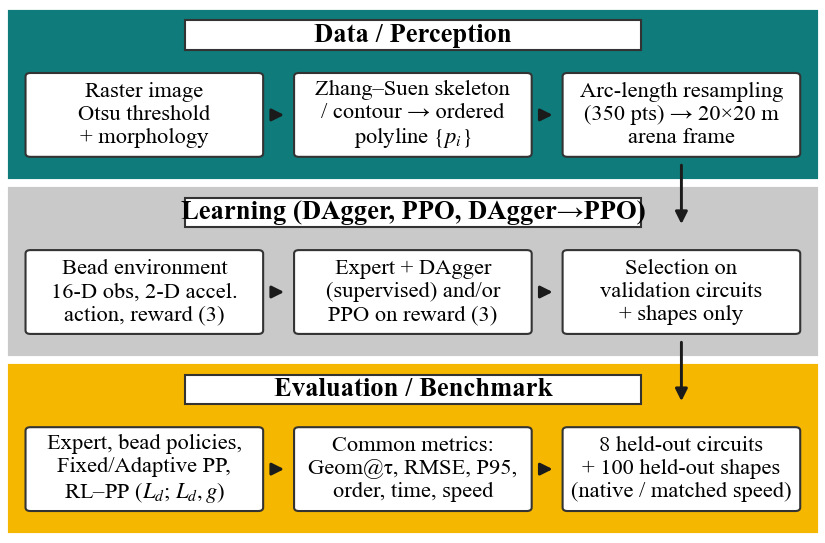
\includegraphics[width=\columnwidth]{fig1_pipeline.png}
\caption{System overview. Top: an input picture is turned into an ordered reference path. Middle: the bead network is trained with DAgger, with PPO, or with DAgger and then PPO, and checkpoints are picked on validation paths only. Bottom: the bead policies, the geometric expert and the Pure Pursuit family, including our rebuild of RL-tuned PP~\cite{elgouhary2026}, are scored with the same measures on unseen circuits and shapes.}
\label{fig:pipeline}
\end{figure}

\subsection{Raster-to-Reference Perception}\label{sec:perception}
Images larger than 1200~px on their longest side are scaled down, then converted to gray levels and smoothed with a Gaussian filter. Otsu's method~\cite{otsu1979} separates the drawing from the background; whether the drawing is darker or lighter is decided from the median brightness along the image border, so either convention works. Small holes are filled by a $3\times3$ closing. When the drawing covers no more than 20\% of the image it is treated as a thin stroke and reduced to a one-pixel skeleton by Zhang--Suen thinning~\cite{zhang1984}; larger regions are traced along their outer contours instead. Every 8-connected piece of the skeleton is converted into an ordered list of points by walking from an end pixel and, wherever the stroke branches, continuing in the direction that turns least. The points are scaled into a $20\times20$~m arena with the vertical axis flipped to obtain a right-handed frame, pieces shorter than 0.1~m are dropped, and the rest are resampled at equal arc-length spacing, about 350 points in total shared in proportion to length. The junctions between separate pieces are stored as breaks and skipped in every distance computation. An image from which no path can be obtained is now reported as a failure; previously the code quietly replaced it with a default circle, and this fallback is switched off for all experiments.

Because every circuit image is rasterized from a known centerline, the extraction error can be measured exactly. Over all 23 circuits the mean distance from the source centerline to the extracted reference is \VextMeanLo--\VextMeanHi~cm per circuit and the maximum is \VextMax~cm. This error is of the same order as the tracking errors reported below; all tracking metrics are therefore measured against the extracted reference, not against the true centerline. Fig.~\ref{fig:inputs} shows the front end on four kinds of input.
\begin{figure}[t]
\centering
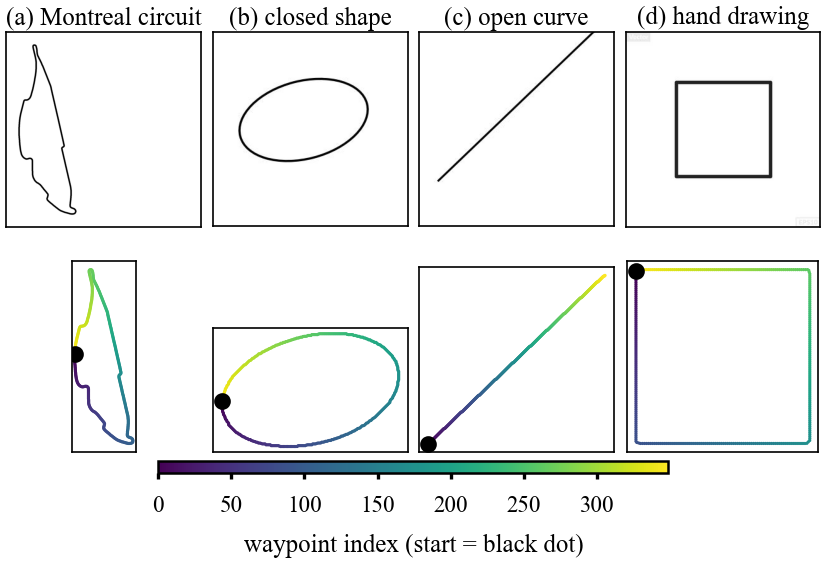
\includegraphics[width=\columnwidth]{fig8_inputs.png}
\caption{Image-to-reference front end. Top: raster inputs---a rasterized test circuit, a closed shape and an open curve from the synthetic test splits, and a hand-drawn image. Bottom: the ordered references extracted from them, colored by waypoint index; the black dot marks waypoint 0.}
\label{fig:inputs}
\end{figure}


\subsection{Bead Dynamics}\label{sec:dyn}
We model the bead as a disc of radius 0.15~m whose state is its position $\mathbf{p}_t\in\mathbb{R}^2$ and velocity $\mathbf{v}_t$. The command $\mathbf{u}_t\in[-1,1]^2$ is scaled to an acceleration of at most $a_{\max}=10$~m/s$^2$ along each axis, the motion is slowed by viscous friction $\mu=7$~s$^{-1}$ and limited to $v_{\max}=7$~m/s, and the state is advanced every $\Delta t=0.016$~s:
\begin{equation}
\begin{aligned}
\mathbf{v}_{t+1}&=(\mathbf{v}_t+a_{\max}\mathbf{u}_t\Delta t)(1-\mu\Delta t),\\
\mathbf{p}_{t+1}&=\mathbf{p}_t+\mathbf{v}_{t+1}\Delta t,
\end{aligned}\label{eq:dyn}
\end{equation}
where speeds above $v_{\max}$ are clipped and the bead rebounds from the arena boundary with a restitution coefficient of 0.15. Holding a full command along one axis drives (\ref{eq:dyn}) to the steady speed
\begin{equation}
v^{*}=a_{\max}\Delta t\,(1-\mu\Delta t)/(\mu\Delta t)\approx1.27~\text{m/s},\label{eq:vstar}
\end{equation}
while a full diagonal command gives at most $\sqrt2\,v^{*}\approx1.79$~m/s; in practice the friction, rather than $v_{\max}$, limits how fast the bead can go. An episode is truncated after $\max(3500,\lceil1.5L/(v^{*}\Delta t)\rceil)$ steps for a reference of length $L$, so that a bead moving at $v^{*}$ can always finish (the earlier fixed cap of 3500 steps could not cover the longest circuits), or after 400 consecutive steps without progress. The same cap is applied to the PP vehicle.

\subsection{Observation and Action Spaces}
The policy receives a 16-element vector $\mathbf{o}_t$ whose entries lie in $[-1,1]$, expressed relative to the bead and divided by the arena half-width $N=10$~m. Its entries are: the vectors to the current and following waypoints (4 values); the scaled position (2) and velocity (2); the distance to the closest reference point searched within $\pm20$ indices (1); a flag telling whether the bead is on the path (1); the cosines of the direction of motion (2); a signed turning-angle measure of the local curvature (1); the unit vector to the waypoint five steps ahead (2); and the fraction of the path completed (1). The output is the 2-D acceleration command $\mathbf{u}_t$. The waypoint counter $w_t$ can move forward by at most four indices per step and only to points within the coverage radius $\rho=0.18$~m, so the bead cannot skip ahead where the path doubles back near itself.

\subsection{Reward Design}
Writing $e_t$ for the distance to the closest reference point, $d_t$ for the distance to waypoint $w_t$, $n_t$ for the number of waypoints passed in the current step, and $\hat{\mathbf{r}}_t$ for the unit tangent of the path, the reward at each step is
\begin{align}
r_t={}&w_a\,\mathrm{clip}\big((d_{t-1}-d_t)/\rho,-1,1\big)+w_w n_t\nonumber\\
&+w_e\exp[-(e_t/\sigma)^2]\nonumber\\
&+w_\tau\,\mathrm{clip}(\mathbf{v}_t\cdot\hat{\mathbf{r}}_t/v_{\max},-1,1)-w_\ell\min(e_t/\rho_s,3)\nonumber\\
&-w_o\mathbb{1}[e_t>\rho]-w_b\mathbb{1}_{\mathrm{back}}-w_c\mathbb{1}_{\mathrm{wall}}\nonumber\\
&-w_j\min(\|\mathbf{u}_t-\mathbf{u}_{t-1}\|,1)-w_s,\label{eq:reward}
\end{align}
in which $\mathbb{1}_{\mathrm{back}}$ flags a step backward along the path, $\mathbb{1}_{\mathrm{wall}}$ flags contact with the boundary, $\sigma=0.08$~m is the width of the Gaussian bonus for staying centered, and $\rho_s=0.10$~m is the tight tolerance. At the end of an episode the agent gains $+50$ if the waypoint counter reached 99\% of the path, $+15$ if the episode was cut off after passing 80\%, and $-5$ in every other case. The weights, kept from the earlier version, appear in Table~\ref{tab:weights}. In this version the reward is the training signal of the PPO variants (Section~\ref{sec:learning}); the DAgger variant does not use it.

\begin{table}[t]
\centering
\caption{Reward Weights of the Bead Environment}
\label{tab:weights}
\setlength{\tabcolsep}{3.5pt}
\begin{tabular}{lcc|lcc}
\toprule
Term & Symbol & Weight & Term & Symbol & Weight\\
\midrule
Approach & $w_a$ & 0.10 & Off-curve & $w_o$ & 0.10\\
Waypoint & $w_w$ & 0.40 & Backtrack & $w_b$ & 0.05\\
Centering & $w_e$ & 0.25 & Wall contact & $w_c$ & 0.50\\
Tangency & $w_\tau$ & 0.15 & Action jerk & $w_j$ & 0.005\\
Tracking error & $w_\ell$ & 0.05 & Step cost & $w_s$ & 0.001\\
\bottomrule
\end{tabular}
\end{table}

\subsection{Policy Architecture and Learning}\label{sec:learning}
We use the actor--critic of Stable-Baselines3~\cite{raffin2021}, giving the actor and the critic their own two-layer networks of 256 tanh units and using a diagonal Gaussian over actions whose spread does not depend on the state. At test time the mean action is applied, with no sampling. The hand-written teacher simply steers toward the waypoint after the current one,
\begin{equation}
\mathbf{u}^{*}_t=(\mathbf{p}[w_t+1]-\mathbf{p}_t)/\|\mathbf{p}[w_t+1]-\mathbf{p}_t\|.\label{eq:expert}
\end{equation}
The same network is trained in three ways, which we name by the procedure that actually updates it.

\textbf{Bead-DAgger} first fits the actor to one teacher-driven episode on each training path and then improves it with DAgger~\cite{ross2011}: the network drives, the teacher supplies the correct action for every state reached, and the growing dataset is fitted with a squared-error loss on the actor branch (Algorithm~\ref{alg:dagger}). Neither the critic nor the reward plays any part.

\textbf{Bead-PPO} optimizes the network from a random initialization with the clipped surrogate objective of PPO~\cite{schulman2017},
\begin{equation}
\mathcal{L}(\theta)=\mathbb{E}_t\big[\min(\varrho_t\hat A_t,\mathrm{clip}(\varrho_t,1\pm\epsilon)\hat A_t)\big]-c_v\mathcal{L}^{V}+c_e\mathcal{H},\label{eq:ppo}
\end{equation}
where $\varrho_t$ is the probability ratio between the new and the rollout policy, $\hat A_t$ is the GAE~\cite{schulman2016} advantage of the reward (\ref{eq:reward}), $\mathcal{L}^{V}$ the value loss and $\mathcal{H}$ the policy entropy. Time-limit truncations are bootstrapped with the critic. The hyper-parameters (Table~\ref{tab:hyper}) are those declared for the network in the earlier version, where they were never exercised; the only addition, the initial log standard deviation, was chosen from $\{-1,-0.5,0\}$ by a validation-only pilot with a seed that is not reported.

\textbf{Bead-DAgger$\to$PPO} copies the actor of the Bead-DAgger checkpoint of the same seed, trains the critic for $5\times10^4$ steps with the actor frozen, and then continues with (\ref{eq:ppo}) under the same settings and the same step budget as Bead-PPO.

All three variants sample training references from the training split, with circuits making up about half of all episodes, and keep the checkpoint with the best validation score: the mean Geom@0.10 minus the mean RMSE in meters, averaged with equal weight over validation circuits and validation shapes. No test reference is used before the final evaluation.

\begin{algorithm}[t]
\caption{Expert anchoring and DAgger refinement (Bead-DAgger)}
\label{alg:dagger}
\begin{algorithmic}[1]
\STATE \textbf{Input:} training references $\mathcal{T}$, validation references $\mathcal{V}$, expert $\pi^{*}$ (\ref{eq:expert}), network $\pi_\theta$, mixing schedule $\beta=(0.4,0.2,0.1,0.05,0,0,0,0)$
\STATE $\mathcal{D}\leftarrow$ one expert episode per $\tau\in\mathcal{T}$; fit actor on $\mathcal{D}$ (12 epochs, lr $2\times10^{-4}$)
\FOR{round $k=1,\dots,8$}
\STATE for each $\tau\in\mathcal{T}$, roll out one episode executing $\pi^{*}$ w.p.\ $\beta_k$, else $\pi_\theta$; label every state with $\pi^{*}(o)$
\STATE $\mathcal{D}\leftarrow\mathcal{D}\cup\{(o,\pi^{*}(o))\}$; refit actor (8 epochs, lr $1.5\times10^{-4}$ for $k\le3$, else $7\times10^{-5}$)
\STATE evaluate the validation score on $\mathcal{V}$; keep the checkpoint if it improves
\ENDFOR
\STATE \textbf{return} best validation checkpoint
\end{algorithmic}
\end{algorithm}

\begin{table}[t]
\centering
\caption{Learning Hyperparameters}
\label{tab:hyper}
\resizebox{\columnwidth}{!}{%
\begin{tabular}{lcc}
\toprule
Quantity & Bead (PPO variants) & RL--PP (re-impl.\ of~\cite{elgouhary2026})\\
\midrule
Policy / value MLP & $[256,256]$ tanh & SB3 default $[64,64]$\\
Rollout $n_{\mathrm{steps}}$ / batch & 2048$\times$4 envs / 128 & 2048 / 256\\
Epochs per update & 10 & 5\\
$\gamma$ / GAE $\lambda$ & 0.99 / 0.95 & 0.99 / 0.98\\
Clip $\epsilon$ / target KL & 0.2 / -- & 0.2 / 0.015\\
Entropy / value coeff. & 0.001 / 0.5 & 0.02 / 0.6\\
Grad-norm clip & 0.5 & 0.7\\
Learning rate & $3\times10^{-4}$ & $2.4\times10^{-4}$, linear decay\\
Initial $\log\sigma$ & $-0.5$ (pilot-selected) & 0 (default)\\
Normalization & -- & VecNormalize (obs, return)$^{\ddagger}$\\
Environment steps & $4\times10^5$ per run & $10^5$ per run\\
Training seeds & 0, 1 & 0, 1\\
\bottomrule
\multicolumn{3}{l}{\footnotesize $^{\ddagger}$Statistics saved with each checkpoint and applied at evaluation.}
\end{tabular}}
\end{table}

\subsection{Re-implementation of RL-Tuned Pure Pursuit}\label{sec:rlpp}
To give both controllers the same paths and the same scoring, we rebuilt the method of~\cite{elgouhary2026} in our arena. The car is simulated with a kinematic bicycle model~\cite{rajamani2012} of wheelbase $W=0.33$~m. PP takes the sideways offset $y'$ of the lookahead point in the car's own frame, converts it into a desired curvature, and turns that curvature into a steering angle:
\begin{equation}
\begin{aligned}
&\gamma=g\cdot2y'/L_d^2,\qquad \dot\theta=(v/W)\tan\delta,\\
&\delta=\mathrm{clip}(\arctan(W\gamma),\pm1.10~\mathrm{rad}),
\end{aligned}\label{eq:pp}
\end{equation}
As in~\cite{elgouhary2026}, the agent sees the speed, the curvature magnitudes $\kappa_{0,1,2}$ at $0$, $5$ and $12$ waypoints ahead, and their difference $\Delta\kappa=\kappa_1-\kappa_0$; we add the signed sideways error and the sine and cosine of the heading error, for eight inputs in total. Its two outputs are mapped to $L_d\in[0.20,1.20]$~m and $g\in[0.60,1.40]$ and then low-pass filtered as in~\cite{elgouhary2026}, with $\beta_L=\beta_g=0.2$:
\begin{equation}
\begin{aligned}
\tilde L_{t+1}&=\beta_L L_{t+1}+(1-\beta_L)\tilde L_t,\\
\tilde g_{t+1}&=\beta_g g_{t+1}+(1-\beta_g)\tilde g_t.
\end{aligned}\label{eq:smooth}
\end{equation}
Our arena is several times smaller than a real F1TENTH track, so the original parameter ranges and teacher constants had to be scaled down. The teacher's targets are $L^{*}=\mathrm{clip}(0.65-0.18\kappa_{\max}+0.04v,\,0.26,\,0.85)$ and $g^{*}=\mathrm{clip}(0.96+0.14\kappa_{\max},\,0.60,\,1.40)$. Speed follows a friction-limited target $v_{\mathrm{ref}}=\mathrm{clip}(4.2/\sqrt{1+2.5|\kappa|},1.8,5.0)$~m/s, smoothed by a backward braking pass (3.5~m/s$^2$) and a forward acceleration pass (2.5~m/s$^2$), and the car tracks it with $a=3(v_{\mathrm{ref}}-v)$. The reward contains the terms of~\cite{elgouhary2026}---closeness to the teacher, penalties on abrupt parameter changes, a curvature-dependent lookahead term, and terms for progress, speed, collisions and stalling, clipped to $[-30,100]$---plus three additions: a Gaussian corridor bonus $3.5\exp[-\frac12(e/0.035)^2]$, a quadratic penalty for errors above 0.07~m, and an alignment bonus $0.8\cos e_\theta$. The joint and the $L_d$-only RL--PP agents are now trained independently, whereas the earlier version took the $L_d$-only controller from the joint network's output.

Two classical controllers complete the set: Fixed PP with constant $(L_d,g)$ and Adaptive PP with $L_d=\mathrm{clip}(a+bv,0.20,1.20)$, $g=1.05$. Both were grid-searched on the training references ($16\times6$ and $9\times6$ grids) with the same selection score as the learned controllers. Fixed PP selects $(L_d,g)=(\VfixL\ \mathrm{m},\VfixG)$, and Adaptive PP selects $(a,b)=(\VadA,\VadB)$, i.e.\ a constant lookahead at the 0.20~m lower bound. Both optima lie on a boundary of the search space. The original gains $(0.55\ \mathrm{m},1.05)$ and schedule $(0.35,0.25)$ are reported alongside.

\section{Experimental Setup}
\subsection{References and Datasets}
We rasterized all 23 circuits of the public F1TENTH racetrack collection\footnote{\url{https://github.com/f1tenth/f1tenth_racetracks}, commit b95c4ef.} with the same 1200-px, 7-px-stroke procedure as before (the three images of the earlier version are reproduced bit-identically) and passed them through the front end of Section~\ref{sec:perception}. Hockenheim, Montreal, and Yas Marina, the circuits of the earlier version, were assigned to the test split; the remaining 20 were split by a seeded permutation, fixed before any training, into 5 further test, 4 validation, and 11 training circuits (Fig.~\ref{fig:split}). No circuit appears in more than one split. Training additionally uses 60 closed shapes and 60 open curves from the training splits of two synthetic datasets of 1000 images each (polygons, ellipses, and rounded quadrilaterals; arcs, lines, and parabolas); 25 of each validation split are used for selection and the first 50 of each test split for testing. Synthetic splits are i.i.d.\ draws from the same generator, so they test in-distribution generalization; the circuits test transfer to unseen layouts. In total \VnRefs~references were passed through the front end---23 circuits, 120 training, 50 validation and all 300 test-split synthetic contours---and all were extracted without failure; of the 300 synthetic test references, the first 50 per set (\VnSynthEval) were evaluated.

\begin{figure}[t]
\centering
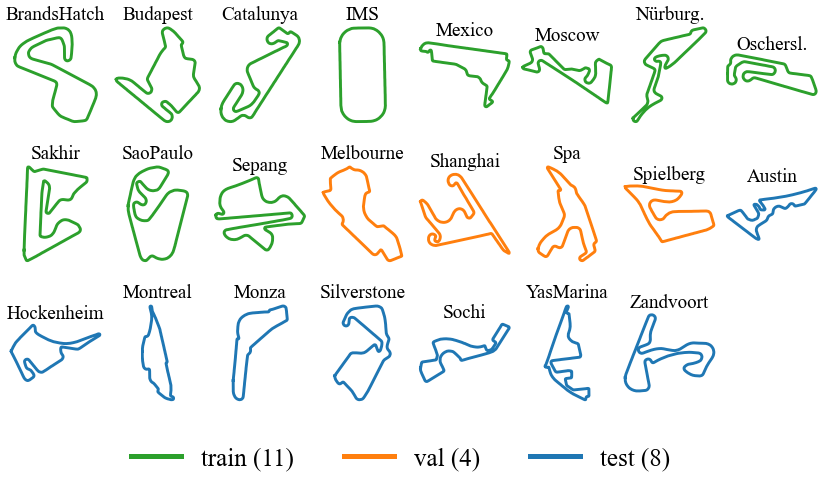
\includegraphics[width=\columnwidth]{fig2_split.png}
\caption{Extracted references of the 23 F1TENTH circuits, colored by split. The test split contains the three circuits of the earlier version (Hockenheim, Montreal, Yas Marina) and five further circuits; no test circuit is used for training, checkpoint selection, or baseline tuning.}
\label{fig:split}
\end{figure}

\subsection{Metrics}
For a reference $P=(\mathbf{p}_0,\dots,\mathbf{p}_{N-1})$ and a driven trajectory $X=(\mathbf{x}_0,\dots,\mathbf{x}_T)$, geometric coverage with tolerance $\tau$ is the share of reference points lying within $\tau$ of the trajectory polyline:
\begin{equation}
\mathrm{Geom@}\tau=\frac1{N}\sum_{\mathbf{p}\in P}\mathbb{1}[\mathrm{dist}(\mathbf{p},X)\le\tau].\label{eq:geom}
\end{equation}
In the other direction, the distance $E=\mathrm{dist}(\mathbf{x},P)$ of each trajectory sample from the reference gives the root-mean-square tracking error (RMSE), its 95th percentile (P95) and its maximum. Geom@$\tau$ does not care about the order of visits. Ordered coverage $K/N$ counts the largest set of reference points $i_1<\dots<i_K$ that are each visited, $\|\mathbf{x}_{t_k}-\mathbf{p}_{i_k}\|\le\rho$, at non-decreasing times $t_1\le\dots\le t_K$; dynamic programming evaluates it exactly, and it punishes skipped or reversed sections while still crediting the remainder of a lap after a single excursion. We count a run as completed when its ordered coverage is 0.95 or more. A single piece of code computes every measure from the saved trajectories of all controllers, whereas the earlier version scored the bead and the car with two different progress rules. Lap time equals the number of steps times $\Delta t$.

\subsection{Protocol}
Every controller was executed for five episodes per test circuit with seeds $\{50000+137k\}$, $k=0,\dots,4$, which perturb the initial position by up to $\pm5$~cm, and for one episode per test shape. Policies were run deterministically. Each learned controller was trained with two seeds, a number limited by our compute budget; Table~\ref{tab:circuits} reports the mean over seeds with the range across seeds in brackets. Track~A runs each controller at its native pace; Track~B caps the PP reference speed at $v_{\mathrm{match}}=1.256$~m/s, the mean speed of the expert on the training circuits, with Fixed and Adaptive PP re-tuned and RL--PP retrained at that speed. Pre-declared comparisons are paired over the 8 test circuits: an exact two-sided Wilcoxon signed-rank test with Holm correction over 14 tests, and the mean paired difference with a 95\% bootstrap interval that resamples circuits and training seeds. With $n=8$ the smallest attainable two-sided $p$ is 0.0078. Table~\ref{tab:circuits} lists 15 controllers; counting each training seed separately they form \VnInst~evaluated instances: 9 controllers with a single instance (the expert, the six classical PP configurations, and the two published checkpoints) and 6 learned controllers with two seeds each (Bead-DAgger, Bead-PPO, Bead-DAgger$\to$PPO, RL--PP joint, RL--PP $L_d$ only, RL--PP joint at $v_{\mathrm{match}}$). Each instance ran $8\times5=40$ circuit episodes and \VnSynthEval~contour episodes, giving $\VnInst\times140=\VnEpisodes$ test episodes, executed on a CPU-only workstation using PyTorch~2.11, Stable-Baselines3~2.8~\cite{raffin2021}, and Gymnasium~1.2~\cite{towers2024}. For verification, every metric was recomputed from the stored trajectories, RMSE and Geom@0.10 additionally with an independent implementation, twelve controller instances were re-executed from their saved checkpoints with bit-identical trajectories, and all tables were regenerated from the raw records; the scripts are part of the released code.

\section{Results and Discussion}
This section starts with accuracy on the unseen circuits, then looks at the effect of PPO on the bead (Section~\ref{sec:ppo}), at the balance between precision and speed (Section~\ref{sec:pace}) and at the synthetic contours (Section~\ref{sec:zero}). It continues with the schedule learned by RL--PP (Sections~\ref{sec:interp}--\ref{sec:abl}) and ends with the threats to validity.

\begin{table*}[t]
\centering
\caption{Tracking Performance on the Eight Held-Out Test Circuits (Mean over Circuits, Five Episodes Each; Learned Controllers: Mean over Two Training Seeds with the Range across Seeds in Brackets; Best Accuracy per Column in Bold; Time and Speed Not Ranked)}
\label{tab:circuits}
\footnotesize
\setlength{\tabcolsep}{3.2pt}
\resizebox{\textwidth}{!}{%
\begin{tabular}{lccccccccc}
\toprule
Controller & Geom@0.05 [\%]\,$\uparrow$ & Geom@0.10 [\%]\,$\uparrow$ & RMSE [cm]\,$\downarrow$ & P95 [cm]\,$\downarrow$ & Max [cm]\,$\downarrow$ & Ordered [\%]\,$\uparrow$ & Completed [\%] & Time [s] & Speed [m/s]\\
\midrule
\tabinput tables/tab_circuits.tex 
\bottomrule
\multicolumn{10}{l}{$^\ast$Checkpoint of the earlier version; trained and selected on Hockenheim, Montreal and Yas Marina, which are three of the eight test circuits here.}\\
\multicolumn{10}{l}{$^\dagger$Checkpoint of the earlier version (trained on one hand-drawn contour); evaluated on raw observations as in that version, because its normalization statistics were not saved.}
\end{tabular}}
\end{table*}

\subsection{Circuit-Level Tracking Accuracy}
Table~\ref{tab:circuits} and Fig.~\ref{fig:bars} consolidate the held-out circuit results. Among the bead controllers, \textbf{Bead-DAgger matches its geometric expert almost exactly} (RMSE \VrmseDagger~vs.\ \VrmseExpert~cm, Geom@0.10 99.1\% vs.\ 99.2\%), with negligible difference between its two seeds. Both PPO variants are worse: Bead-DAgger$\to$PPO reaches \VrmseDP~cm and Bead-PPO from scratch \VrmsePPO~cm, the latter covering only \VgPPO\% of the reference within 0.10~m and completing \VcompPPO\% of the test runs. The published checkpoint of the earlier version reaches \VrmsePubBead~cm on these circuits; on the three circuits it was trained on, it reproduces the earlier figures (Table~\ref{tab:paper}).

\textbf{The PP family is at least as accurate.} Tuned Fixed PP reaches \VrmseFix~cm and tuned Adaptive PP \VrmseAd~cm, both below the expert and every bead policy, while traversing a lap in \VtFix~s instead of \VtExpert~s. Retrained RL--PP reaches \VrmseRL~cm. The gap between these values and the earlier version is explained by two corrections: with the original gains Fixed PP reaches \VrmseFixOrig~cm, and the published RL--PP checkpoint, evaluated on unnormalized observations, \VrmsePubRL~cm. Geom@0.10 is about one point lower for every PP controller than for the expert (98.2\% vs.\ 99.2\%). On every test circuit the only reference points left beyond 0.10~m by tuned Fixed PP and by the expert are the last waypoints before the start/finish line: the PP lap-completion rule ends an episode six to seven waypoints before loop closure and the bead's 99\% rule three. Geom@$\tau$ differences of this size are therefore an artifact of episode termination, not of tracking. Ordered coverage is at least 97.9\% and every PP run is completed.

Fig.~\ref{fig:traces} shows complete laps on the three circuits of the earlier version, and Fig.~\ref{fig:cdf} the distribution of the lateral error over all test circuits: the expert, Bead-DAgger, RL--PP and both tuned PP laws keep at least 96.9\% of the trajectory samples within 3~cm of the reference, against 65.8\% for Bead-DAgger$\to$PPO and 40.5\% for Bead-PPO.
\begin{figure}[t]
\centering
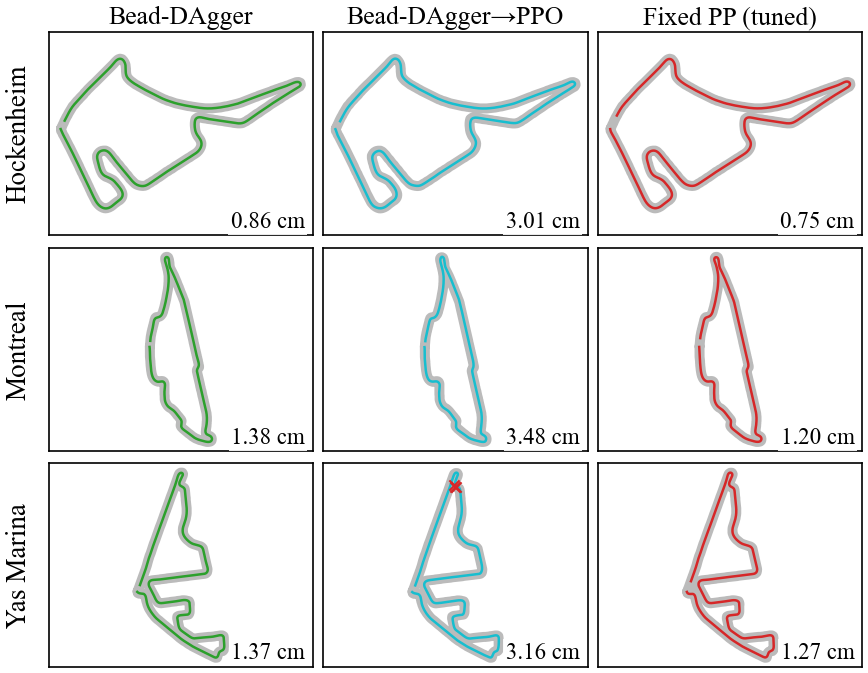
\includegraphics[width=\columnwidth]{fig9_traces.png}
\caption{Full-lap trajectories on the three circuits of the earlier version, now held out (first episode, training seed 0), over the reference (grey). Red crosses: reference points left farther than 0.10~m, excluding the start/finish closure. Inset: tracking RMSE of the lap.}
\label{fig:traces}
\end{figure}

\begin{figure}[t]
\centering
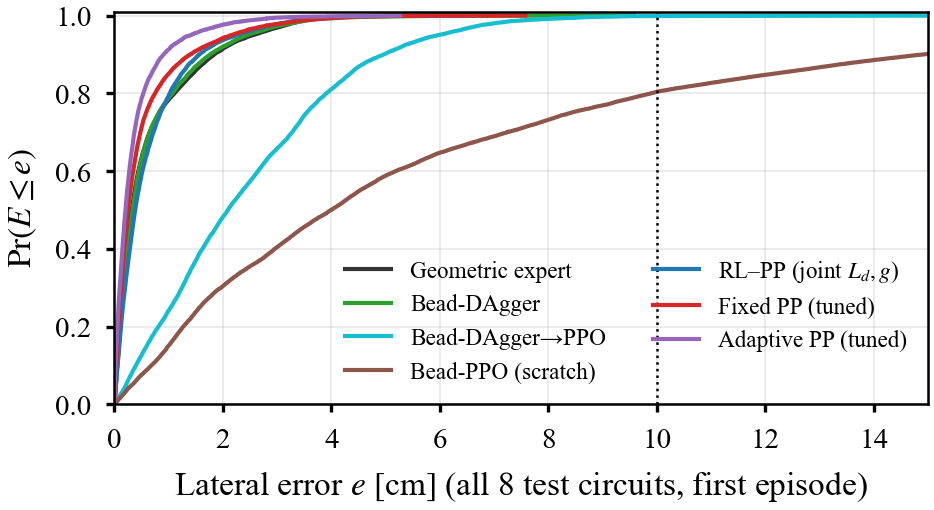
\includegraphics[width=\columnwidth]{fig11_cdf.png}
\caption{Cumulative share of trajectory samples below a given distance from the reference, pooled over the eight test circuits (first episode, training seed 0 where applicable). Dotted line: 0.10~m.}
\label{fig:cdf}
\end{figure}

Fig.~\ref{fig:zoom} shows where the bead policies fail. At the Montreal corners where Bead-DAgger$\to$PPO deviates most, it rounds the corner exit, whereas the expert, Bead-DAgger, tuned Fixed PP and RL--PP follow nearly coincident paths; Bead-PPO from scratch cuts the corner.

\begin{figure}[t]
\centering
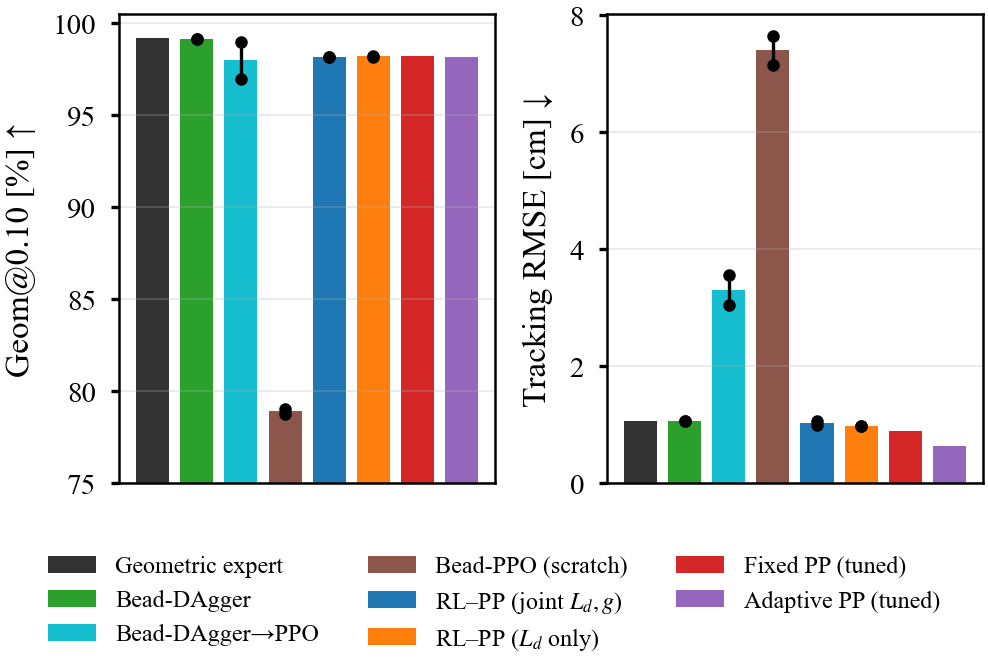
\includegraphics[width=\columnwidth]{fig3_bars.png}
\caption{Mean Geom@0.10 (left; larger is better) and RMSE (right; smaller is better) over the eight test circuits. Each dot is one training seed of a learned controller.}
\label{fig:bars}
\end{figure}

\begin{figure}[t]
\centering
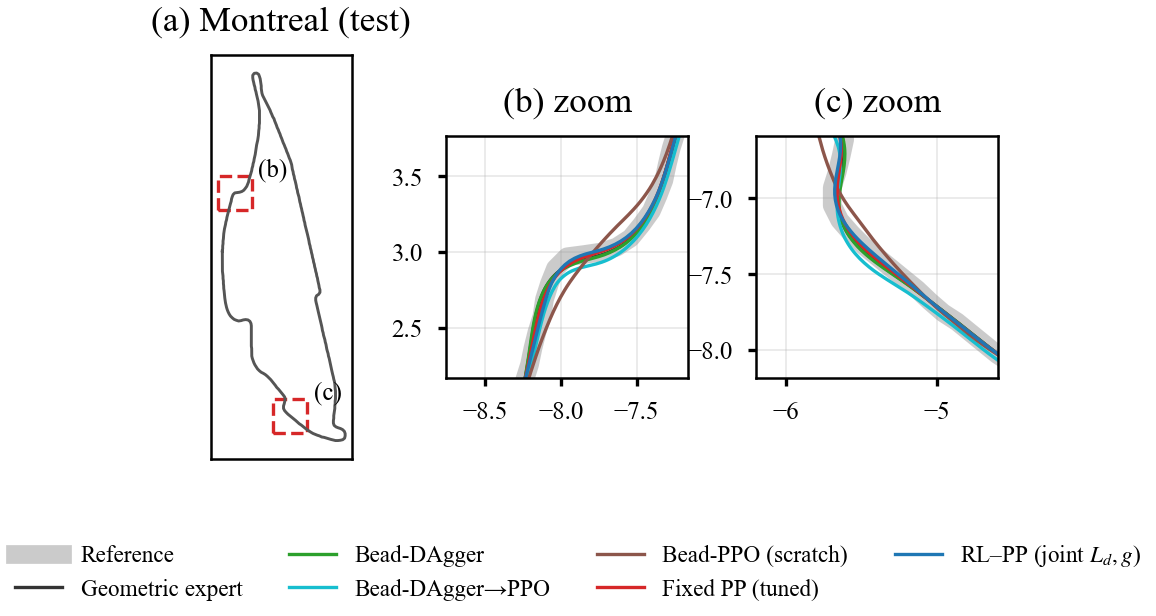
\includegraphics[width=\columnwidth]{fig6_zoom.png}
\caption{Qualitative comparison on the held-out Montreal circuit (first episode, training seed 0). The zoom windows are centered, automatically, on the two reference points that Bead-DAgger$\to$PPO misses by the largest distance, excluding the start/finish region.}
\label{fig:zoom}
\end{figure}

\subsection{What PPO Does to the Bead Policy}\label{sec:ppo}
The PPO variants are genuinely optimized on the reward (\ref{eq:reward}): actor, critic and action noise are all updated (verified by unit tests, including the exact transfer of the DAgger actor and its freezing during the critic warm-up, where the approximate KL divergence stayed below $10^{\VfrozenKLexp}$). The training diagnostics are unremarkable: the final approximate KL per update lies between \VklLo~and \VklHi, and the critic's explained variance reaches \VevLo--\VevHi. The validation error of Bead-PPO falls monotonically for both seeds, from about 10.8 to 8.0~cm over $4\times10^5$ steps (Fig.~\ref{fig:learning}). The budget was too small for convergence; the selected configuration was still improving when its validation-only pilot was stopped at $7.5\times10^5$ steps. PPO fine-tuning of Bead-DAgger did not improve it: the validation error rose from 0.87~cm to 3.5--4.2~cm at the first evaluation after the critic warm-up and stayed between 3.0 and 4.3~cm.

On the test circuits the deterministic policies rank the same by reward and by accuracy: the expert earns the highest cumulative reward (\VrewExpert), Bead-DAgger nearly the same (\VrewDagger), Bead-DAgger$\to$PPO less (\VrewDP), and Bead-PPO least (\VrewPPO). PPO did, however, optimize a stochastic policy, so we ran a validation-only diagnostic: each policy was executed on the four validation circuits with and without Gaussian action noise of the standard deviation used by PPO (three noise seeds, two training seeds). Averaged over seeds, deterministic Bead-DAgger earns \VdiagDagDetrew~(RMSE \VdiagDagDetrmse~cm, \VdiagDagDett~s); with PPO's initial noise it earns \VdiagDagStorew~(\VdiagDagStormse~cm, \VdiagDagStot~s). After fine-tuning, the policy earns \VdiagDPStorew~with its own noise and \VdiagDPDetrew~without (\VdiagDPDetrmse~cm, \VdiagDPDett~s). Two conclusions follow. First, \textbf{within the budget, PPO fine-tuning lowered rather than raised the return of the very stochastic policy it optimizes} on held-out circuits, so the loss of accuracy is not a mismatch between stochastic training and deterministic evaluation; the episode rewards logged during training rose, but they mix references of very different length and are not comparable across iterations. Second, \textbf{the reward (\ref{eq:reward}) is not monotone in accuracy}: the noisy DAgger policy is three times less accurate and slower, yet earns more, because the centering bonus is paid at every step and a slower traversal collects it for longer. Even a fully converged PPO policy would therefore not necessarily maximize tracking accuracy. Which factor---learning rate, the mixture of circuits and short contours in training, critic error, or the budget---caused the fine-tuning to degrade the policy was not isolated. We report this as a negative result: under our settings, reward-driven fine-tuning did not refine the imitation policy, and the expert is the accuracy ceiling of every bead variant evaluated here.

\begin{figure}[t]
\centering
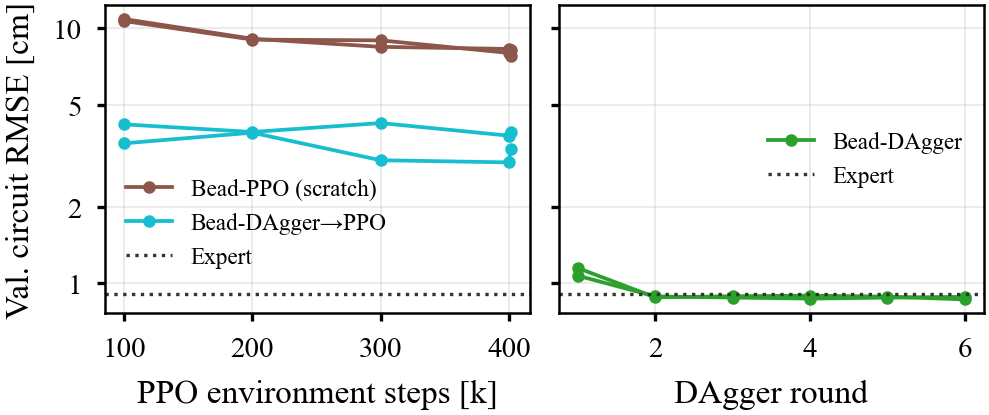
\includegraphics[width=\columnwidth]{fig5_learning.png}
\caption{Validation-circuit RMSE during training (two seeds each). Left: PPO from scratch and DAgger-initialized PPO. Right: DAgger rounds (stopped after six of eight rounds; the score was flat from round 2). Dotted: geometric expert on the same validation circuits.}
\label{fig:learning}
\end{figure}

\subsection{The Precision--Pace Trade-off}\label{sec:pace}
A bead lap lasts roughly $2.3$ times as long as a lap of the PP car at its own speed (Fig.~\ref{fig:pace}). This gap comes from the dynamics: according to (\ref{eq:vstar}), friction holds the bead near 1.3~m/s per axis, while the car follows a speed plan that reaches 5~m/s on straights. The earlier version already warned that accuracy cannot be compared fairly at different speeds, and Track~B addresses this. When the car's target speed is limited to $v_{\mathrm{match}}$, its lap time becomes close to the bead's (Table~\ref{tab:circuits}) and its error drops a little further: \VrmseFixM~cm for re-tuned Fixed PP, \VrmseAdM~cm for Adaptive PP and \VrmseRLM~cm for retrained RL--PP. \textbf{At matched speed, the bicycle-model PP controllers track the extracted references more closely than every bead controller, including the expert.}

\begin{figure}[t]
\centering
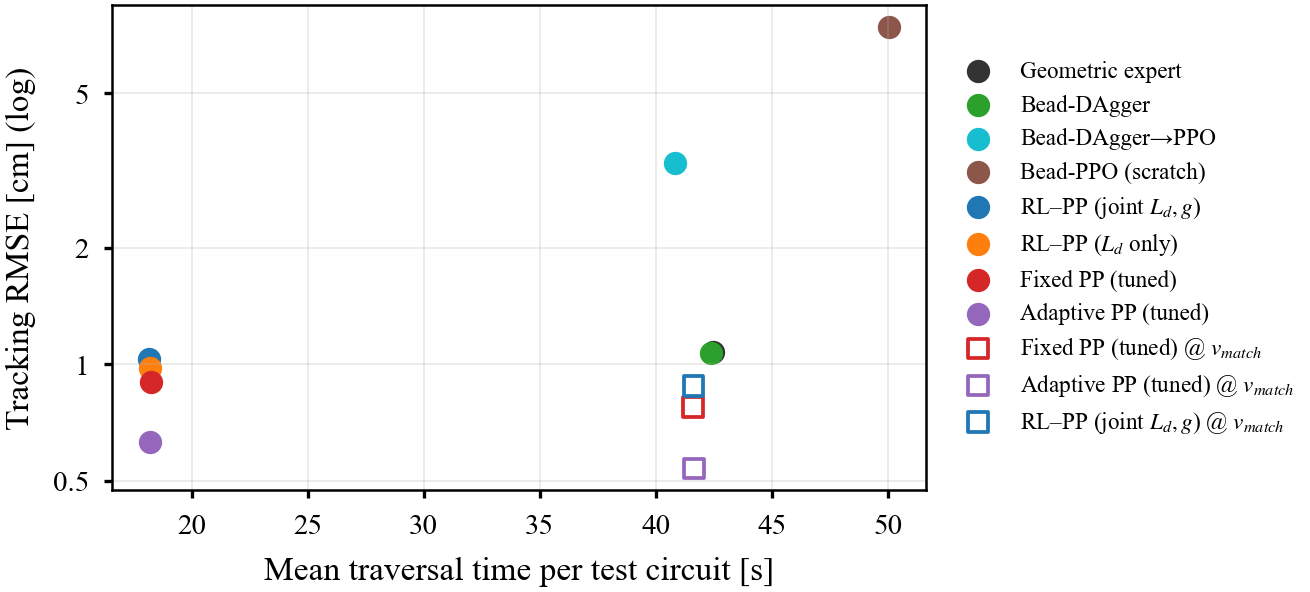
\includegraphics[width=\columnwidth]{fig4_pace.png}
\caption{Precision versus pace on the test circuits. Filled circles: native speed (Track~A). Open squares: PP controllers with the reference speed capped at $v_{\mathrm{match}}$ (Track~B).}
\label{fig:pace}
\end{figure}

\subsection{Generalization to Held-Out Contours}\label{sec:zero}
Table~\ref{tab:shapes} reports the 100 synthetic test contours. Every controller except Bead-PPO from scratch and the two published checkpoints exceeds 98\% Geom@0.10 on both sets; the expert, Bead-DAgger and tuned Fixed PP all lie between 1.0 and 1.2~cm RMSE. On short, simple contours the metric ceiling is reached by every adequate controller, and the ranking among them is within a few millimeters.

\begin{table}[t]
\centering
\caption{Results on Held-Out Synthetic Test Contours (Mean $\pm$ Standard Deviation across Contours; Best per Set in Bold)}
\label{tab:shapes}
\footnotesize
\setlength{\tabcolsep}{3pt}
\resizebox{\columnwidth}{!}{%
\begin{tabular}{lcccc}
\toprule
Set / Controller & Geom@0.10 [\%] & RMSE [cm] & Ordered [\%] & Time [s]\\
\midrule
\tabinput tables/tab_shapes.tex 
\bottomrule
\end{tabular}}
\end{table}

\subsection{Interpretability of the Learned PP Schedule}\label{sec:interp}
Fig.~\ref{fig:interp} shows how the retrained joint RL--PP agent sets its parameters on Montreal. The lookahead uses the whole allowed interval, \VrlppLmin--\VrlppLmax~m, and falls as the upcoming curvature rises ($r=\VrLk$), matching the trend described in~\cite{elgouhary2026}: the agent looks closer before corners and farther on straights. Unlike in the earlier version, where the gain stayed within $0.96\le g\le1.04$, the steering gain now varies between \VrlppGmin~and \VrlppGmax~(standard deviation \VrlppGstd) and increases in corners ($r=+\VrGk$), as the teacher prescribes. The difference coincides with the correction of the observation normalization.

\begin{figure}[t]
\centering
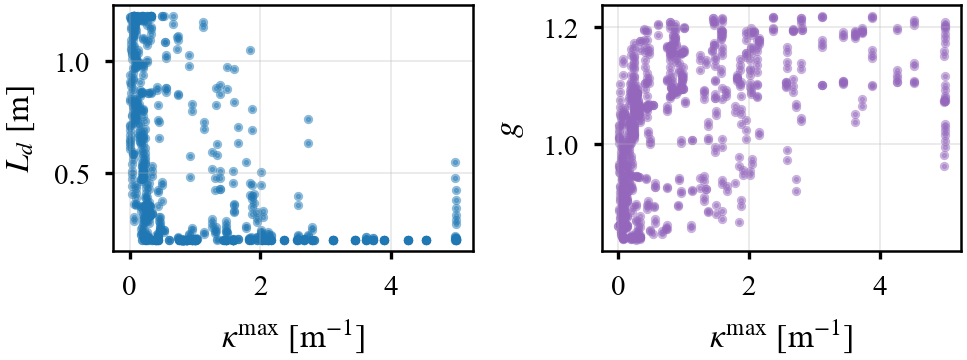
\includegraphics[width=\columnwidth]{fig7_interp.png}
\caption{Learned joint RL--PP schedule on the held-out Montreal circuit (training seed 0): $L_d$ (left) and $g$ (right) versus previewed curvature $\kappa_{\max}$.}
\label{fig:interp}
\end{figure}

\subsection{Ablation: Joint versus Lookahead-Only Tuning}\label{sec:abl}
This time the $L_d$-only agent was trained on its own, so the ablation concerns training and not only inference as before. Dropping the gain output still makes no difference: the $L_d$-only agent is very slightly more accurate than the joint one (Table~\ref{tab:comp}), and neither beats tuned Fixed PP. In our small arena and with our budget, learned PP parameters therefore offered no advantage over good constant ones; this says nothing against the hardware results of~\cite{elgouhary2026}.

\begin{table*}[t]
\centering
\caption{Pre-Declared Paired Comparisons on the Eight Test Circuits (Difference A$-$B; RMSE Lower and Geom@0.10 Higher is Better for A)}
\label{tab:comp}
\footnotesize
\resizebox{\textwidth}{!}{%
\begin{tabular}{llcccccc}
\toprule
Comparison (A vs B) & Metric & Mean diff. & 95\% bootstrap CI & A better on & Wilcoxon $p$ & Holm $p$\\
\midrule
\tabinput tables/tab_comparisons.tex 
\bottomrule
\end{tabular}}
\end{table*}

\subsection{Statistical Evidence}
Table~\ref{tab:comp} lists the pre-declared comparisons. Several effects are consistent across all eight circuits---DAgger$\to$PPO is less accurate than DAgger, than the expert, and than tuned Fixed PP at either speed on every circuit---and their bootstrap intervals exclude zero. Their unadjusted $p=0.0078$ is, however, the smallest value attainable with eight circuits, and after Holm correction over 14 tests \textbf{none reaches 0.05}. We therefore describe these differences as consistent but not statistically established. The two-seed intervals reflect only a minimal sample of training variability.

\begin{table}[t]
\centering
\caption{Geom@0.10 [\%] / RMSE [cm] on the Three Circuits of the Earlier Version (Now Held Out; Best per Column in Bold)}
\label{tab:paper}
\footnotesize
\setlength{\tabcolsep}{2.5pt}
\resizebox{\columnwidth}{!}{%
\begin{tabular}{lcccccc}
\toprule
& \multicolumn{2}{c}{Hockenheim} & \multicolumn{2}{c}{Montreal} & \multicolumn{2}{c}{Yas Marina}\\
Controller & G@0.10 & RMSE & G@0.10 & RMSE & G@0.10 & RMSE\\
\midrule
\tabinput tables/tab_paper_circuits.tex 
\bottomrule
\end{tabular}}
\end{table}

\subsection{Threats to Validity}
We revisit the limitations of the earlier version and add new ones. (i)~Training exposure and (ii)~model selection: resolved; no test circuit is used for training, checkpoint selection, or tuning. The test circuits were, however, known to the authors when the reward and the network were designed in the earlier version. (iii)~The dynamics differ: partly addressed; Track~B matches speed, but the bead remains holonomic and the PP vehicle non-holonomic. (iv)~Actor-only training: resolved; PPO now optimizes actor and critic on the reward, but with $4\times10^5$ steps it is under-trained, and its fine-tuning hyper-parameters were not tuned. (v)~Single models: partly addressed; two training seeds instead of one, which bounds rather than estimates seed variance. (vi)~Scale and hardware: unchanged; all results are in simulation at arena scale, no physical experiments were performed, and the RL--PP ranges and teacher were rescaled from~\cite{elgouhary2026}. New: (vii)~reference-extraction error (up to \VextMax~cm) is of the same order as the reported tracking errors; (viii)~the tuned PP optima lie on a boundary of their grids, so the PP baselines may be further improvable; (ix)~DAgger was stopped after six of eight rounds and only 50 of 150 synthetic test contours per set were used, both for compute reasons; (x)~synthetic test contours share their generator with the training contours; (xi)~the reward (\ref{eq:reward}) pays a per-step centering bonus and therefore favors slower traversal (Section~\ref{sec:ppo}), so it is an imperfect proxy for the accuracy metrics; (xii)~the PPO conclusions hold for one hyper-parameter configuration, $4\times10^5$ steps and two seeds, and do not establish that PPO cannot reach expert-level accuracy on this task.

\section{Conclusion}
This work tested, under shared paths and shared measures, whether a network that commands actuation directly can out-track a PP controller with learned parameters. The direct controller was a point-mass bead fed by an image-to-path front end and trained with DAgger, with PPO, or with both in sequence; the comparison set consisted of our rebuild of RL-tuned PP~\cite{elgouhary2026} and two classical PP controllers.

\textbf{With test circuits held out and all baselines tuned on training data, the answer is no.} The DAgger-trained bead reproduces its geometric expert to within a millimeter, so the direct-actuation accuracy is the expert's, not a product of learning. PPO, applied to the same reward, did not improve on that expert within our budget, either from scratch or as fine-tuning; a validation diagnostic shows that fine-tuning lowered even the return it optimizes, and that the reward itself rewards slow traversal more than accuracy. A Fixed PP with tuned gains tracks more closely at more than twice the pace, and more closely still at matched speed. Retrained RL--PP reproduces the qualitative lookahead behavior of~\cite{elgouhary2026}, and now also a curvature-dependent gain, but is not more accurate than tuned Fixed PP. These differences are consistent across circuits but not statistically established with two seeds and eight circuits.

These limitations suggest the next steps: (a)~running PPO much longer, with more seeds and tuned fine-tuning settings, to find out whether reward-based learning can surpass the teacher; (b)~redesigning the reward so that its shaping terms do not accumulate with episode length and centimeter-scale errors outweigh progress; (c)~testing a pursuit-style law on the bead itself, to separate the effect of the dynamics from that of the controller; (d)~making path extraction more accurate than the tracking errors being measured; and (e)~deploying the bead policy on a real F1TENTH car as a path generator for a lower-level steering controller.

\section*{Acknowledgment}
We are grateful to the F1TENTH community for publishing its track data, and to Elgouhary and El-Wakeel~\cite{elgouhary2026}, whose detailed description of their method allowed us to rebuild it in our simulator.

\begin{thebibliography}{00}
\bibitem{okelly2020} M. O'Kelly, H. Zheng, D. Karthik, and R. Mangharam, ``F1TENTH: An open-source evaluation environment for continuous control and reinforcement learning,'' in \textit{Proc. NeurIPS 2019 Competition and Demonstration Track}, PMLR vol. 123, 2020, pp. 77--89.
\bibitem{coulter1992} R. C. Coulter, ``Implementation of the pure pursuit path tracking algorithm,'' Carnegie Mellon Univ., Robotics Inst., Tech. Rep. CMU-RI-TR-92-01, 1992.
\bibitem{snider2009} J. M. Snider, ``Automatic steering methods for autonomous automobile path tracking,'' Carnegie Mellon Univ., Robotics Inst., Tech. Rep. CMU-RI-TR-09-08, 2009.
\bibitem{elgouhary2026} M. Elgouhary and A. S. El-Wakeel, ``Learning to tune pure pursuit in autonomous racing: Joint lookahead and steering-gain control with PPO,'' arXiv:2602.18386, 2026.
\bibitem{schulman2017} J. Schulman, F. Wolski, P. Dhariwal, A. Radford, and O. Klimov, ``Proximal policy optimization algorithms,'' arXiv:1707.06347, 2017.
\bibitem{ross2011} S. Ross, G. J. Gordon, and J. A. Bagnell, ``A reduction of imitation learning and structured prediction to no-regret online learning,'' in \textit{Proc. AISTATS}, 2011, pp. 627--635.
\bibitem{hoffmann2007} G. M. Hoffmann, C. J. Tomlin, M. Montemerlo, and S. Thrun, ``Autonomous automobile trajectory tracking for off-road driving: Controller design, experimental validation and racing,'' in \textit{Proc. American Control Conf.}, 2007, pp. 2296--2301.
\bibitem{rajamani2012} R. Rajamani, \textit{Vehicle Dynamics and Control}, 2nd ed. New York, NY, USA: Springer, 2012.
\bibitem{kong2015} J. Kong, M. Pfeiffer, G. Schildbach, and F. Borrelli, ``Kinematic and dynamic vehicle models for autonomous driving control design,'' in \textit{Proc. IEEE Intelligent Vehicles Symp.}, 2015, pp. 1094--1099.
\bibitem{heilmeier2020} A. Heilmeier, A. Wischnewski, L. Hermansdorfer, J. Betz, M. Lienkamp, and B. Lohmann, ``Minimum curvature trajectory planning and control for an autonomous race car,'' \textit{Vehicle System Dynamics}, vol. 58, no. 10, pp. 1497--1527, 2020.
\bibitem{betz2022} J. Betz \textit{et al.}, ``Autonomous vehicles on the edge: A survey on autonomous vehicle racing,'' \textit{IEEE Open J. Intell. Transp. Syst.}, vol. 3, pp. 458--488, 2022.
\bibitem{kiran2022} B. R. Kiran \textit{et al.}, ``Deep reinforcement learning for autonomous driving: A survey,'' \textit{IEEE Trans. Intell. Transp. Syst.}, vol. 23, no. 6, pp. 4909--4926, 2022.
\bibitem{kober2013} J. Kober, J. A. Bagnell, and J. Peters, ``Reinforcement learning in robotics: A survey,'' \textit{Int. J. Robotics Research}, vol. 32, no. 11, pp. 1238--1274, 2013.
\bibitem{schulman2016} J. Schulman, P. Moritz, S. Levine, M. Jordan, and P. Abbeel, ``High-dimensional continuous control using generalized advantage estimation,'' in \textit{Proc. ICLR}, 2016.
\bibitem{andrychowicz2021} M. Andrychowicz \textit{et al.}, ``What matters in on-policy reinforcement learning? A large-scale empirical study,'' in \textit{Proc. ICLR}, 2021.
\bibitem{haarnoja2018} T. Haarnoja, A. Zhou, P. Abbeel, and S. Levine, ``Soft actor-critic: Off-policy maximum entropy deep reinforcement learning with a stochastic actor,'' in \textit{Proc. ICML}, 2018, pp. 1861--1870.
\bibitem{evans2023} B. D. Evans, H. W. Jordaan, and H. A. Engelbrecht, ``Comparing deep reinforcement learning architectures for autonomous racing,'' \textit{Machine Learning with Applications}, vol. 14, p. 100496, 2023.
\bibitem{pomerleau1989} D. A. Pomerleau, ``ALVINN: An autonomous land vehicle in a neural network,'' in \textit{Advances in Neural Information Processing Systems 1}, 1989, pp. 305--313.
\bibitem{otsu1979} N. Otsu, ``A threshold selection method from gray-level histograms,'' \textit{IEEE Trans. Syst., Man, Cybern.}, vol. 9, no. 1, pp. 62--66, 1979.
\bibitem{zhang1984} T. Y. Zhang and C. Y. Suen, ``A fast parallel algorithm for thinning digital patterns,'' \textit{Commun. ACM}, vol. 27, no. 3, pp. 236--239, 1984.
\bibitem{raffin2021} A. Raffin, A. Hill, A. Gleave, A. Kanervisto, M. Ernestus, and N. Dormann, ``Stable-Baselines3: Reliable reinforcement learning implementations,'' \textit{J. Mach. Learn. Res.}, vol. 22, no. 268, pp. 1--8, 2021.
\bibitem{towers2024} M. Towers \textit{et al.}, ``Gymnasium: A standard interface for reinforcement learning environments,'' arXiv:2407.17032, 2024.
\end{thebibliography}

\end{document}
